\chapter{DISEÑO DEL PRODUCTO}
\label{cap:diseno}

\section{ARQUITECTURA DEL SISTEMA}
\label{sec:arquitectura}
El desarrollo del problema de optimización exigía un volumen alto de pruebas y experimentos, por lo
que las decisiones de \textit{stack} se tomaron antes de construir el sistema, guiadas por tres
criterios.

\begin{enumerate}
  \item Costo. Se anticipó un volumen elevado de ejecuciones durante el desarrollo y la evaluación
        experimental del sistema. Bajo ese escenario, un componente tarificado por consulta
        convierte cualquier precio unitario en un gasto difícil de acotar. El criterio fue mantener
        en cero el gasto de la etapa de desarrollo. Este criterio califica las alternativas para esa
        etapa; no excluye adoptar más adelante un componente de pago cuyo aporte al producto en
        operación justifique su costo recurrente.
  \item Tiempo de ejecución. Se descartan las latencias que no provienen del trabajo útil: la ida y
        vuelta a un servicio remoto por cada consulta de ruteo, o una implementación que recalcule
        lo ya calculado. El presupuesto de tiempo del sistema se reserva para el trabajo propio del
        problema.
  \item Simplicidad del desarrollo. Entre soluciones de resultado equivalente se prefiere la que
        deja menos piezas que operar y mantener, dado que en la iteración actual del proyecto se
        cuenta con un solo desarrollador. La simplicidad cede cuando la alternativa compleja aporta
        una capacidad que el producto necesita.
\end{enumerate}

Los tres criterios se aplican de forma conjunta, sin un orden de prioridad fijo, y resolvieron la
elección de cada componente: Django con GeoDjango ---la única alternativa evaluada que integra
PostGIS en el ORM---, \textit{OR-Tools} frente a una heurística propia y a los \textit{solvers}
comerciales de licencia recurrente, OSRM frente a las APIs de ruteo tarificadas por consulta,
\textit{React}~18 \citep{react} con Vite y \textit{Leaflet} \citep{leaflet} para la interfaz
cartográfica, Celery con Redis para el trabajo asíncrono, y un monolito modular en lugar de
servicios separados por dominio.\footnote{Ver \hyperref[anx:stack]{Anexo 8}.} El patrón que recorre
esas decisiones es que ninguna se resolvió por rendimiento aislado del componente: donde existía
una alternativa de pago, su aporte no compensaba el gasto proyectado ni la latencia que introduce,
y entre las alternativas libres decidió la simplicidad de operarlas.

La arquitectura resultante sigue el patrón de monolito modular: un único servicio Django
\citep{django} con módulos separados por dominio (\texttt{accounts}, \texttt{datasets},
\texttt{optimization}, \texttt{routes}). Las tareas de optimización se ejecutan de forma asíncrona
mediante Celery \citep{celery} con Redis como \textit{broker}. El motor de ruteo peatonal OSRM
\citep{osrm} se despliega como un contenedor más del propio sistema ---tanto en desarrollo como en
producción (Sección~\ref{sec:despliegue-produccion})--- y procesa datos de \textit{OpenStreetMap}
\citep{openstreetmap} de Chile, lo que elimina costos de API y dependencias de red durante la
optimización. La persistencia geográfica se apoya en la extensión espacial PostGIS de PostgreSQL
\citep{postgis}.

La Ilustración~\ref{fig:arquitectura} resume las capas del sistema y el recorrido de una
optimización: el navegador solicita el trabajo a la API, esta lo encola en Celery en lugar de
resolverlo en el ciclo de la petición HTTP, y el \textit{worker} ejecuta el \textit{pipeline}, que
consulta OSRM para construir la matriz de costos y persiste la solución en PostGIS. La petición
HTTP termina en cuanto los trabajos quedan encolados, de modo que el navegador nunca espera al
\textit{solver}: el \textit{frontend} consulta el estado por \textit{polling} hasta que alcanza un
estado terminal, y un fallo del \textit{worker} deja el trabajo en \texttt{failed} con el mensaje
de la excepción, que el panel muestra sin necesidad de un canal de error distinto del de estado. El
trazo continuo marca las capas del monolito Django; el trazo discontinuo, los servicios
de apoyo desplegados como contenedores independientes.

\begin{figure}[H]
  \centering
  % babel-spanish activa '<' y '>'; sin esto, la punta de flecha (>=stealth) no compila
  \shorthandoff{<>}%
  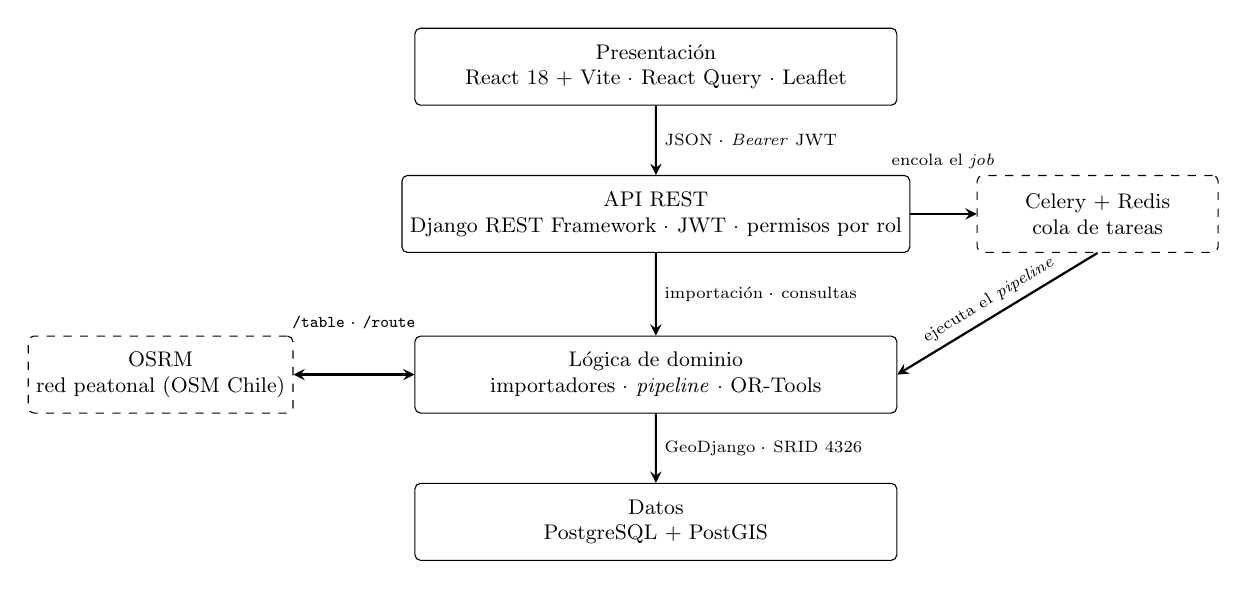
\begin{tikzpicture}[
      scale=0.85, transform shape,
      capa/.style={draw, rounded corners=2pt, align=center, font=\small,
                   minimum width=7.2cm, minimum height=1.15cm},
      externo/.style={draw, dashed, rounded corners=2pt, align=center, font=\small,
                      minimum width=3.6cm, minimum height=1.15cm},
      flujo/.style={->, >=stealth, thick},
      etiqueta/.style={font=\scriptsize, midway}
    ]
    \node[capa]    (p) at (0,0)      {Presentación\\ React 18 + Vite · React Query · Leaflet};
    \node[capa]    (a) at (0,-2.2)   {API REST\\ Django REST Framework · JWT · permisos por rol};
    \node[capa]    (l) at (0,-4.6)
      {Lógica de dominio\\ importadores · \textit{pipeline} · OR-Tools};
    \node[capa]    (d) at (0,-6.8)   {Datos\\ PostgreSQL + PostGIS};
    \node[externo] (q) at (6.6,-2.2) {Celery + Redis\\ cola de tareas};
    \node[externo] (o) at (-7.4,-4.6) {OSRM\\ red peatonal (OSM Chile)};

    \draw[flujo] (p) -- (a) node[etiqueta,right] {JSON · \textit{Bearer} JWT};
    \draw[flujo] (a) -- (l) node[etiqueta,right] {importación · consultas};
    \draw[flujo] (l) -- (d) node[etiqueta,right] {GeoDjango · SRID 4326};
    \draw[flujo] (a.east) -- (q.west) node[etiqueta,above,yshift=0.55cm] {encola el \textit{job}};
    \draw[flujo] (q.south) -- (l.east) node[etiqueta,above,sloped] {ejecuta el \textit{pipeline}};
    \draw[flujo,<->] (l.west) -- (o.east)
      node[etiqueta,above,yshift=0.55cm] {\texttt{/table} · \texttt{/route}};
  \end{tikzpicture}
  \caption{Arquitectura de Arbocensus.}
  \label{fig:arquitectura}
\end{figure}

\subsection{Despliegue de producción}
\label{sec:despliegue-produccion}

Al cierre de la iteración el sistema quedó desplegado en un servidor virtual (\textit{droplet}) de
\textit{DigitalOcean} con Ubuntu 24.04 y 2\,GB de memoria\footnote{Se amplió la memoria con 2\,GB
de intercambio porque el preprocesamiento inicial de OSRM excede la memoria física del servidor.}.
Se descartó una plataforma como servicio ---la vía de iteraciones pasadas del proyecto---: alojar
allí una composición de seis servicios, con OSRM residente en memoria, implica contratar cada pieza
por separado con un costo que crece por servicio, mientras que un servidor virtual único aloja el
conjunto completo a costo fijo. La composición de producción, definida con \textit{Docker Compose}
\citep{merkel2014docker,dockercompose}, declara seis servicios ---PostGIS, Redis, OSRM, la
aplicación Django, el \textit{worker} de Celery y Caddy \citep{caddy}--- con reinicio automático y
verificaciones de salud encadenadas; OSRM opera aquí sobre un extracto de Santiago recortado del de
Chile, lo que permite que el servicio quepa en la memoria del servidor.

Caddy actúa como proxy inverso y único punto de entrada: sirve el paquete estático del
\textit{frontend} y redirige las peticiones de la API a la aplicación Django. El sistema queda
accesible públicamente en \url{https://134.122.20.233.sslip.io}, un dominio derivado de la IP del
servidor que permite operar con TLS ---obtenido y renovado contra \textit{Let's Encrypt}
\citep{letsencrypt}--- mientras el proyecto no fija un dominio propio; como el \textit{frontend} y
la API comparten origen, no se requieren excepciones de CORS, y la aplicación añade archivos
estáticos con huella de contenido, HSTS y \textit{cookies} restringidas a HTTPS. La entrega es
continua: un \textit{push} a la rama \texttt{production} construye las imágenes, las publica
etiquetadas por confirmación y actualiza el servidor por SSH, de modo que volver a una versión
anterior se reduce a redesplegar su etiqueta. Un respaldo diario genera un \textit{dump} de la base
de datos y un archivo con las fotografías, con retención de siete días y sin copia externa, límite
que el Capítulo~\ref{cap:resultados} registra entre las limitaciones vigentes.

% ---- 3.2 -------------------------------------------------------
\section{MODELO DE DATOS}
\label{sec:modelo-datos}

Los modelos de dominio centrales son los siguientes:

\begin{enumerate}
  \item Dataset: agrupa un conjunto de árboles importados desde CSV o desde una fuente legada.
  \item Tree: punto geográfico (\texttt{PointField}, SRID 4326) perteneciente a un \texttt{Dataset}.
        Registra además su procedencia mediante los campos \texttt{source} y \texttt{external\_id},
        que identifican la fuente legada y el identificador que el árbol tenía en ella
        (Sección~\ref{sec:legacy}).
  \item RoutingConfig: parámetros de una sesión de optimización ($T_{\min}$, $T_{\max}$, $s$).
  \item OptimizationJob: tarea de optimización con estado (\texttt{queued}, \texttt{running},
        \texttt{completed}, \texttt{failed}) y referencia a la tarea Celery.
  \item RoutingSolution: resultado de un \texttt{OptimizationJob} para una estrategia de partición
        dada (campo \texttt{strategy}). Almacena el número de rutas $k$, el tiempo total de
        desplazamiento, el puntaje de balance temporal, las métricas espaciales de la solución y el
        desglose de tiempos por fase del \textit{pipeline}; la relación \texttt{participants}
        alimenta el cálculo de carga acumulada por censista (Sección~\ref{sec:ui}).
  \item Route: ruta individual con tiempos estimados; su asignación a un censista 
        (\texttt{surveyor}) es opcional.
  \item RouteStop: visita de un árbol en una ruta, con número de secuencia y estado de
        visita.
  \item TreeObservation: registro histórico del estado de un árbol en un instante dado
        (Sección~\ref{sec:recenso}). Es la entidad que convierte el sistema en una herramienta de
        re-censo y no solo de censo inicial.
  \item DistanceMatrix: caché persistente de la matriz $n \times n$ de tiempos de caminata entre
        árboles obtenida de OSRM (Sección~\ref{sec:matriz}); su cardinalidad 1:1 con
        \texttt{Dataset} refleja que la matriz se cachea una vez por conjunto de árboles activos,
        no una vez por optimización.
\end{itemize}

La procedencia se modela en el propio \texttt{Tree} en lugar de en una entidad aparte, porque solo
se necesita para dos fines: evitar la doble importación de un mismo árbol legado y vincular sus
observaciones históricas. Una restricción de unicidad parcial sobre la terna (\texttt{dataset},
\texttt{source}, \texttt{external\_id}), condicionada a \texttt{external\_id} no nulo, impide que un
mismo árbol legado aparezca dos veces en un \textit{dataset} sin restringir a los árboles importados
desde CSV, que no tienen identificador externo. El orden de visita de cada ruta se deriva de
\texttt{RouteStop.sequence}; no existe un campo redundante de secuencia en \texttt{Route}.

Cada \texttt{OptimizationJob} produce una \texttt{RoutingSolution} por cada estrategia de partición
ejecutada (Sección~\ref{sec:estrategias}), lo que permite comparar los enfoques sobre un mismo
conjunto de árboles. Para gobernar cuál es la vigente en terreno, el modelo incorpora un ciclo de
publicación: el campo \texttt{published\_at} marca la solución activa y una restricción de unicidad
parcial garantiza a lo más una solución publicada por \textit{dataset}; publicar una nueva
despublica atómicamente la anterior, y la asignación de censistas solo se permite sobre la solución
publicada.

La Ilustración~\ref{fig:er} presenta el modelo entidad-relación simplificado. Se omiten los
atributos no estructurales, así como la relación auxiliar que vincula cada observación con el
usuario que la registra: ese campo es anulable por la misma razón que lo es el censista de una ruta.
Todas las entidades usan claves primarias UUID.

\begin{figure}[H]
  \centering
  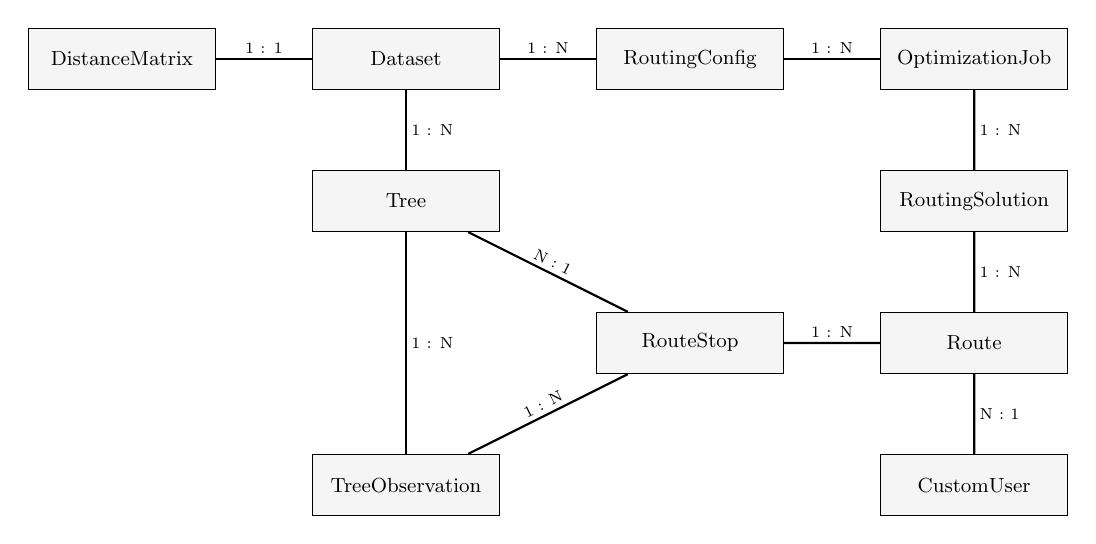
\begin{tikzpicture}[
      scale=0.82, transform shape,
      entidad/.style={draw, fill=black!4, align=center, font=\small,
                      minimum width=2.9cm, minimum height=0.95cm},
      rel/.style={-, thick},
      card/.style={font=\scriptsize, midway, inner sep=2pt}
    ]
    \node[entidad] (dm)  at (-4.4,0)    {DistanceMatrix};
    \node[entidad] (ds)  at (0,0)       {Dataset};
    \node[entidad] (rc)  at (4.4,0)     {RoutingConfig};
    \node[entidad] (job) at (8.8,0)     {OptimizationJob};
    \node[entidad] (tr)  at (0,-2.2)    {Tree};
    \node[entidad] (sol) at (8.8,-2.2)  {RoutingSolution};
    \node[entidad] (rt)  at (8.8,-4.4)  {Route};
    \node[entidad] (rs)  at (4.4,-4.4)  {RouteStop};
    \node[entidad] (obs) at (0,-6.6)    {TreeObservation};
    \node[entidad] (us)  at (8.8,-6.6)  {CustomUser};

    \draw[rel] (ds) -- (dm)  node[card,above] {1 : 1};
    \draw[rel] (ds) -- (rc)  node[card,above] {1 : N};
    \draw[rel] (rc) -- (job) node[card,above] {1 : N};
    \draw[rel] (ds) -- (tr)  node[card,right] {1 : N};
    \draw[rel] (job) -- (sol) node[card,right] {1 : N};
    \draw[rel] (sol) -- (rt) node[card,right] {1 : N};
    \draw[rel] (rt) -- (rs)  node[card,above] {1 : N};
    \draw[rel] (rs) -- (tr)  node[card,above,sloped] {N : 1};
    \draw[rel] (tr) -- (obs) node[card,right] {1 : N};
    \draw[rel] (rs) -- (obs) node[card,above,sloped] {1 : N};
    \draw[rel] (rt) -- (us)  node[card,right] {N : 1};
  \end{tikzpicture}
  \caption{Modelo entidad-relación simplificado.}
  \label{fig:er}
\end{figure}

La doble ruta \texttt{RouteStop} $\to$ \texttt{TreeObservation} y \texttt{Tree} $\to$
\texttt{TreeObservation} del diagrama es lo que permite que una observación de re-censo sobreviva
al plan de rutas que la originó, incluso si esa ruta se reemplaza.

% ---- 3.3 -------------------------------------------------------
\section{MOTOR DE OPTIMIZACIÓN}

% ---- 3.3.1 ------------------------------------------------------
\subsection{Formulación del problema}
\label{sec:formulacion}

\begin{enumerate}
\item Conjuntos, parámetros y variables.

La formulación sigue la estructura estándar de los problemas de ruteo de vehículos
\citep{toth2014vehicle}. El problema se define sobre un conjunto de puntos $P = \{p_1, p_2, \ldots,
p_n\}$ correspondientes a las ubicaciones geográficas de los árboles a censar. Con el propósito de
modelar rutas abiertas ---sin punto de inicio ni de término predefinido---
\citep{li2007open} se añade un depósito ficticio
(\textit{dummy depot}) $p_0$, de modo que el grafo del modelo se define sobre $V = \{0, 1, \ldots,
n\}$, donde el índice $0$ corresponde al depósito y los índices $1$ a $n$ a los árboles reales. Se
dispone de un conjunto $R = \{1, \ldots, N_{\max}\}$ de vehículos, cuyo cardinal es una cota
superior calculada por la Ecuación~\ref{eq:nmax} y no el número de rutas de la solución.

La función de costo $c_{ij}$ representa el tiempo de caminata entre los puntos $p_i$ y $p_j$,
calculado sobre la red vial peatonal real mediante OSRM. Los arcos que tocan el depósito tienen
costo nulo, $c_{0j} = c_{i0} = 0$, lo que es precisamente el mecanismo que abre las rutas: entrar y
salir del depósito es gratuito, de modo que la ruta efectiva es la secuencia de árboles que hay
entre ambos extremos. El parámetro $s$ es el tiempo de servicio constante por árbol, y $d_{ij}$ la
distancia de \textit{haversine} \citep{sinnott1984virtues} entre $p_i$ y $p_j$, empleada por la
dimensión geográfica de la
Sección~\ref{sec:estrategias}.

El modelo emplea tres familias de variables de decisión:

\begin{enumerate}
  \item $x_{ijr} \in \{0,1\}$: vale $1$ si el vehículo $r$ recorre el arco
        $(i,j)$ y $0$ en caso contrario.
  \item $u_i \in \{0,1\}$, para $i \in \{1,\ldots,n\}$: vale $1$ si el árbol $p_i$
        queda incluido en el plan y $0$ si la solución lo descarta
        (Sección~\ref{sec:disyunciones}).
  \item $z_r \in \{0,1\}$: vale $1$ si el vehículo $r$ queda activo, esto es, si
        se le asigna al menos un árbol.
\end{enumerate}

A ellas se añaden las variables acumuladas $t_i \geq 0$ de la dimensión temporal, que registran el
tiempo transcurrido al abandonar el nodo $i$, y su análogo $g_i \geq 0$ sobre la dimensión
geográfica.

\item Restricciones.

Las restricciones estructurales son las estándar de la familia: cada árbol incluido en el plan se
visita exactamente una vez ---la restricción de grado, que un árbol descartado ($u_j = 0$) exime de
todo arco entrante---, todo vehículo que entra a un nodo sale de él ---la conservación de flujo---
y cada vehículo activo sale del depósito y regresa a él a lo sumo una vez, lo que liga la variable
de activación $z_r$ con el uso efectivo del vehículo. La dimensión temporal encadena los tiempos
acumulados $t_i$ a lo largo de cada ruta ---el tiempo de servicio se carga al abandonar cada nodo
real, con el depósito ficticio exento---, y su valor terminal es el tiempo total $T_r$ de la ruta
del vehículo $r$: el desplazamiento más el servicio de sus $m_r$ árboles.\footnote{Ver
\hyperref[anx:formulacion]{Anexo 9}.}

La única restricción temporal dura del modelo es la cota superior de la
Ecuación~\ref{eq:time_constraints}, implementada como capacidad de la dimensión:

\begin{equation}
  T_r \leq T_{\max}, \quad \forall r \in R
  \label{eq:time_constraints}
\end{equation}

con valores por defecto $T_{\min} = 2\,\text{h}$ y $T_{\max} = 3\,\text{h}$, parametrizables por el
administrador. La cota inferior $T_{\min}$ no es una restricción del modelo sino un objetivo blando:
se penaliza el déficit en la función objetivo en lugar de prohibirlo, por la razón que se detalla en
la Sección~\ref{sec:solver}. En consecuencia, una solución puede presentar rutas de duración
inferior a $T_{\min}$; el Capítulo~\ref{cap:resultados} las observa en las áreas reales de baja
carga, no en la instancia de referencia.

\item Función objetivo.

El modelo es monobjetivo: los tres propósitos enunciados más abajo se escalarizan en una suma
ponderada de seis términos, y no se resuelven de forma lexicográfica ni se construye un frente de
Pareto ---el conjunto de soluciones en que ningún objetivo puede mejorar sin empeorar otro---. La
función que el \textit{solver} minimiza es

\begin{equation}
  \begin{aligned}
    \min \quad
      &\underbrace{\sum_{r \in R} \sum_{(i,j)}
        \left\lceil c_{ij} + s\cdot\mathbf{1}[i \neq 0] \right\rceil x_{ijr}}_{\text{costo de arco}}
      \;+\; \underbrace{C_{\text{fijo}} \sum_{r \in R} z_r}_{\text{flota}} \\[2pt]
      &+\; \underbrace{\alpha \sum_{r \in R}
        \max\!\left(0,\; T_{\min} - T_r\right)}_{\text{penalización inferior}}
      \;+\; \underbrace{\beta \sum_{r \in R}
        \max\!\left(0,\; T_r - \tau\right)}_{\text{penalización superior}} \\[2pt]
      &+\; \underbrace{\pi \sum_{i=1}^{n} \left(1 - u_i\right)}_{\text{descarte}}
      \;+\; \underbrace{\lambda_{\text{span}} \sum_{r \in R}
        \operatorname{span}_r}_{\text{extensión geográfica}}
  \end{aligned}
  \label{eq:objetivo}
\end{equation}

donde $\operatorname{span}_r = \max_i g_i - \min_i g_i$ sobre los nodos del vehículo $r$ es la
extensión de la ruta en la dimensión geográfica, y las constantes toman los valores de la
Tabla~\ref{tab:coeficientes}. Las penalizaciones inferior y superior se aplican, en la
implementación, sobre la variable acumulada del nodo terminal de cada vehículo, que es donde $t_i$
vale $T_r$; un vehículo inactivo no contribuye a ninguno de los seis términos.

\small
\begin{xltabular}{\textwidth}{@{}l p{2.2cm} l X@{}}
  \caption{Coeficientes de la función objetivo en producción.}
  \label{tab:coeficientes} \\
  \addlinespace
  \toprule
  Símbolo & Término & Valor & Unidad y lectura \\
  \addlinespace
  \midrule
  \endfirsthead
  \toprule
  Símbolo & Término & Valor & Unidad y lectura \\
  \addlinespace
  \midrule
  \endhead
  \bottomrule
  \endlastfoot
    --- &
      Costo de arco &
      $1$ &
      Por segundo de tránsito. \\
      \addlinespace
    $C_{\text{fijo}}$ &
      Costo fijo de vehículo &
      $100\,000$ &
      Por vehículo activo (Sección~\ref{sec:flota}). \\
      \addlinespace
    $\alpha$ &
      Penalización inferior &
      $10\,000$ &
      Por segundo en que $T_r$ queda bajo $T_{\min}$. \\
      \addlinespace
    $\beta$ &
      Penalización superior &
      $500$ &
      Por segundo en que $T_r$ supera el objetivo blando $\tau$. \\
      \addlinespace
    $\tau$ &
      Objetivo blando superior &
      $(T_{\min}+T_{\max})/2$ &
      Punto medio del intervalo de jornada, en segundos. \\
      \addlinespace
    $\pi$ &
      Penalización de descarte &
      $10^{6}$ &
      Por árbol excluido, esto es $10\,C_{\text{fijo}}$ (Sección~\ref{sec:disyunciones}). \\
      \addlinespace
    $\lambda_{\text{span}}$ &
      Coeficiente de extensión geográfica &
      $3$ &
      Por metro de extensión en la dimensión de \textit{haversine}
      (Sección~\ref{sec:estrategias}). \\
\end{xltabular}
\normalsize

Los tres propósitos que la Ecuación~\ref{eq:objetivo} escalariza son:

\begin{enumerate}
  \item Minimizar el número de rutas $k = \sum_r z_r$, a través del término de flota.
  \item Minimizar el tiempo total de desplazamiento, a través del costo de arco.
  \item Reducir el desbalance de carga entre rutas, a través de las dos penalizaciones blandas que
        empujan cada $T_r$ hacia el intervalo $[T_{\min},\,\tau]$.
\end{enumerate}

Corresponde precisar el tercero, porque su enunciado usual ---«minimizar la desviación estándar de
$T_r$»--- no describe lo que el modelo hace. Una desviación estándar es una propiedad del conjunto
de rutas y no se puede expresar como costo aditivo por arco, que es la única forma que admite la
formulación: el \textit{solver} evalúa un costo por cada arco recorrido y por cada variable
acumulada terminal, nunca un estadístico de la solución completa. Lo que el modelo implementa son
las dos penalizaciones blandas bilaterales de la Ecuación~\ref{eq:objetivo}, y lo que el
Capítulo~\ref{cap:resultados} reporta como balance es un tercer objeto, el cociente
$\min_r T_r / \max_r T_r$. Los tres ---objetivo declarado, mecanismo implementado y métrica
reportada--- apuntan en la misma dirección, pero no son la misma cantidad, y en esta memoria se
nombran por separado.

En la taxonomía de la investigación operativa \citep{toth2014vehicle}, el modelo combina tres
extensiones sobre el \textit{Multiple Travelling Salesman Problem}
\citep{bektas2006multiple,laporte1992traveling}: rutas abiertas ---el \textit{Open Vehicle Routing
Problem} \citep{li2007open}, obtenidas aquí con el depósito ficticio de costo nulo---, visitas
opcionales penalizadas ---la familia \textit{prize-collecting}
\citep{balas1989prize,feillet2005traveling}--- y una dimensión acumulativa con capacidad dura
$T_{\max}$, estructuralmente una restricción de capacidad aunque su unidad sea el tiempo. La
combinación de varias extensiones sobre un mismo modelo es lo que la literatura reciente denomina
un problema de ruteo multiatributo \citep{vidal2013heuristics}.

La escala relativa de los coeficientes importa más que sus valores absolutos, y conviene leerla en
términos marginales, esto es, como el precio de un segundo adicional de caminata en una ruta. Con
los valores por defecto, ese precio es de $-9\,999$ mientras la ruta está por debajo de $T_{\min}$
---el \textit{solver} está pagado por alargarla---, de $+1$ entre $T_{\min}$ y el objetivo blando
$\tau$, y de $+501$ por encima de $\tau$. Esa asimetría, y no el costo de arco, es el canal
dominante del objetivo, y explica los resultados de sensibilidad a las penalizaciones de la
Sección~\ref{sec:discusion-calidad}.

\end{enumerate}

% ---- 3.3.2 ------------------------------------------------------
\subsection{Construcción de la matriz de costos}
\label{sec:matriz}

La matriz de costos $C \in \mathbb{R}^{n \times n}$, donde cada fila y cada columna corresponde a
uno de los $n$ árboles del \textit{dataset}, se construye consultando el \textit{endpoint}
\texttt{/table/v1/foot} de OSRM \citep{osrm}, que devuelve los tiempos de caminata reales entre
todos los pares de puntos en una única solicitud HTTP. El servicio resuelve esas consultas sobre el
grafo de \textit{OpenStreetMap} preprocesado con el algoritmo \textit{Multi-Level Dijkstra}, que
particiona la red en niveles jerárquicos y precalcula atajos entre celdas, lo que permite responder
consultas de camino mínimo en tiempo prácticamente independiente de la longitud del trayecto
\citep{delling2017customizable}.

Con el fin de evitar recomputaciones costosas, la matriz se persiste en el modelo
\texttt{DistanceMatrix} asociado al \textit{dataset}. La clave de caché es un \textit{hash} SHA-256
\citep{sha256} calculado sobre los identificadores de los árboles activos ordenados; si el conjunto
de árboles cambia, el \textit{hash} no coincide y la matriz se recalcula automáticamente.

Los nodos inalcanzables (devueltos como \texttt{null} por OSRM) se reemplazan por una penalización
de $9\,999\,999$ segundos, lo que garantiza la viabilidad numérica del \textit{solver}: la matriz
queda sin valores nulos y toda operación aritmética sobre ella está definida. La sustitución sí
altera la topología de la solución, y esa es justamente su función: un arco de ese costo excede
cualquier cota de jornada concebible, de modo que ninguna ruta puede incorporarlo y el nodo afectado
termina descartado por la disyunción que lo cubre (Sección~\ref{sec:disyunciones}). Lo que la
penalización evita no es el cambio de topología sino la propagación de valores nulos al modelo.

El factor que limita el tamaño de una consulta no es el parámetro \texttt{--max-table-size} de OSRM
(fijado en $5\,000$), sino la longitud máxima de la URL (RE-01): sobre unas $350$ coordenadas
---una veintena de caracteres cada una--- la ruta de la petición se aproxima al límite práctico de
$8$\,kB de los servidores HTTP. Cuando el \textit{dataset} supera ese tope, la matriz se construye
por fragmentación (\textit{chunking}) en bloques de $175$ coordenadas ---la mitad del tope, dado
que cada petición fragmentada transporta las coordenadas del bloque origen y las del destino---, y
el número de solicitudes crece como el cuadrado del número de bloques, porque cada bloque de origen
se consulta contra cada bloque de destino: para los $1\,607$ árboles de la instancia de referencia,
$10 \times 10$ bloques producen $100$ solicitudes, lo que domina el costo de la primera
construcción de la matriz (Capítulo~\ref{cap:resultados}). Un tope adicional de $2\,000$ árboles
acota la dimensión de la matriz, cuyo almacenamiento en JSON crece como $O(n^2)$.

% ---- 3.3.3 ------------------------------------------------------
\subsection{Estimación del número de rutas}

\label{sec:flota}

El número de rutas $k$ ---y por lo tanto el número de censistas que deben salir a terreno en una
jornada--- no es un dato de entrada del sistema: es una salida del \textit{solver}. El administrador
nunca declara cuántos equipos tiene disponibles; declara cuánto puede durar una jornada ($T_{\min}$,
$T_{\max}$) y cuánto toma censar un árbol ($s$), y el sistema deriva la flota necesaria. Derivar $k$
del \textit{solver} evita el enfoque de iteración externa ---resolver el modelo con
$1, 2, 3, \ldots$ vehículos hasta hallar el menor valor factible---, que multiplica el tiempo de
cómputo por el número de intentos y resulta frágil, dado que una corrida infactible no distingue
entre «faltan vehículos» y «el modelo no admite solución».

El tiempo de servicio $s$, en cambio, sí es un dato de entrada, y es un parámetro y no una constante
del sistema porque el protocolo de censo no está fijado de una campaña a otra: el número de
fotografías y de preguntas que un censista completa por árbol varía según lo que la campaña exija
registrar, y esa variación es la que $s$ traslada al modelo. Esa indefinición no es un detalle de
calibración sino una cuestión abierta del proyecto, que la Sección~\ref{sec:recenso} retoma al
discutir qué evidencia exige cada observación en terreno.

En su lugar, el sistema entrega a \textit{OR-Tools} un techo $N_{\max}$ de vehículos disponibles y
deja que el \textit{solver} decida cuántos activa. El techo se calcula a partir del trabajo total
estimado ---servicio más desplazamiento--- dividido por la duración mínima de una ruta:

\begin{equation}
  N_{\max} = \min\!\left(n,\;
  \left\lceil \frac{n \cdot s + n \cdot \hat{c}_{\text{nn}}}{T_{\min}} \right\rceil + b
  \right)
  \label{eq:nmax}
\end{equation}

donde $n$ es el número de árboles activos, $s$ el tiempo de servicio por árbol y
$\hat{c}_{\text{nn}}$ el tiempo medio al vecino más cercano: el promedio, sobre todos los nodos, del
arco de menor costo que sale de cada nodo, excluyendo la diagonal y los pares inalcanzables
(aquellos con la penalización de $9\,999\,999$\,s). Se emplea el vecino más cercano y no el promedio
de todos los pares porque una ruta real encadena árboles contiguos, no pares arbitrarios: el
promedio general sobreestima el desplazamiento por árbol en un factor que crece con la extensión
geográfica del \textit{dataset}, e inflaría $N_{\max}$ innecesariamente. El término $b$ es un margen
de holgura de $5$ vehículos, que absorbe la subestimación del estimador de vecino más cercano sin
ampliar el espacio de búsqueda de forma apreciable; el mínimo
con $n$ impide que el techo supere el caso degenerado de un árbol por ruta.

$N_{\max}$ es una cota superior, no una predicción: solo debe ser lo bastante amplia como para no
excluir la solución óptima. La minimización efectiva de $k$ ocurre dentro del \textit{solver},
mediante el costo fijo de $100\,000$\,s por vehículo activo (Sección~\ref{sec:solver}): activar una
ruta adicional es tan caro que el \textit{solver} solo lo hace cuando las restricciones temporales
lo obligan. El número de rutas de la solución final es, en la práctica, muy inferior al techo: sobre
los $1\,607$ árboles de la instancia de referencia, con un techo de $N_{\max}=36$ vehículos, el
\textit{solver} activa $25$ rutas (Capítulo~\ref{cap:resultados}).

La misma estimación alimenta un segundo uso, orientado a la planificación operativa y no al
\textit{solver}: el \textit{endpoint} \texttt{GET /api/optimization/estimate/} permite al
administrador consultar, antes de lanzar una optimización, cuántos censistas requeriría un
\textit{dataset} bajo un $T_{\min}$ y un tiempo de servicio dados ---aquí la
Ecuación~\ref{eq:nmax} se evalúa con margen nulo ($b=0$), dado que interesa una estimación ajustada
y no un techo, y sobre la matriz en caché, sin disparar consultas a OSRM---. La misma invocación
comprueba la factibilidad de la configuración mediante \texttt{check\_config}, que distingue
bloqueos ---condiciones que garantizan infactibilidad, como un tiempo de servicio mayor que
$T_{\max}$--- de advertencias ---condiciones de riesgo, como el régimen de relleno: caminata que el
\textit{solver} añade sin visitar árboles, solo para alcanzar el piso de jornada---, de modo que el
administrador detecta configuraciones problemáticas antes de lanzar la optimización.

% ---- 3.3.4 ------------------------------------------------------
\subsection{\textit{Solver} VRP con \textit{OR-Tools}}
\label{sec:solver}

La formulación en \textit{OR-Tools} \citep{ortools} usa el modelo de ruteo vehicular
(\textit{Vehicle Routing Problem}, VRP). Los elementos ya descritos se materializan de forma
directa: el depósito ficticio ocupa el nodo $0$ con costo de tránsito cero y los nodos reales se
indexan de $1$ a $n$; $T_{\max}$ se impone como capacidad dura de la dimensión temporal
(\texttt{AddDimension}); el costo fijo de $100\,000$ por vehículo activo materializa la
minimización de flota; y cada árbol puede quedar fuera de la solución a un costo de $1\,000\,000$
(Sección~\ref{sec:disyunciones}). Dos decisiones se fijan en esta capa:

\begin{itemize}[label=--]
  \item Cotas blandas de la dimensión temporal: la cota inferior $T_{\min}$ se implementa mediante
        \texttt{SetCumulVarSoftLowerBound} en el nodo terminal de cada vehículo, con coeficiente
        $10\,000$, porque una cota inferior dura volvería el modelo infactible cuando el número de
        rutas necesarias multiplicado por $T_{\min}$ supera el trabajo disponible; la formulación
        blanda penaliza el déficit en lugar de prohibirlo. \texttt{SetCumulVarSoftUpperBound}
        dirige a su vez las rutas hacia el punto medio $(T_{\min} + T_{\max})/2$, lo que reduce la
        varianza entre rutas.
  \item Búsqueda local: estrategia GLS \citep{voudouris1999guided} con solución inicial
        \textit{PATH\_CHEAPEST\_ARC} ---una construcción voraz por arco más barato, de la misma
        familia que el clásico algoritmo de ahorros \citep{clarke1964scheduling}---. El GLS carece
        de criterio de término por convergencia demostrada (RE-04), de modo que fijar un límite de
        tiempo no es una decisión de diseño sino una condición que la metaheurística impone; lo que
        sí es decisión de diseño es su valor. A falta de un valor explícito, el \textit{pipeline}
        lo deriva del tamaño del problema como $\min(30 + 1{,}5\,n,\ 120)$ segundos, de modo que un
        \textit{dataset} pequeño no consume el presupuesto completo; la expresión satura en su tope
        de $120$\,s a partir de $n = 60$.
\end{itemize}

Si el \textit{solver} no encuentra solución, el \textit{pipeline} emite un error que reporta el
número de árboles y los parámetros de configuración vigentes, de modo que el administrador pueda
identificar qué restricción relajar; esa rama no se activa con la formulación vigente, porque las
disyunciones garantizan siempre una solución, aunque el precio de esa garantía sea descartar
árboles.

% ---- 3.3.5 ------------------------------------------------------
\subsection{Disyunciones de nodos}
\label{sec:disyunciones}

Un modelo VRP en el que todos los nodos son obligatorios puede resultar infactible: basta un único
árbol cuyo tiempo de acceso exceda la cota dura $T_{\max}$ para que no exista asignación válida y
el \textit{solver} retorne sin solución. La situación es realista: los \textit{datasets} provienen
de censos reales y contienen árboles geográficamente aislados, así como nodos que OSRM no logra
enrutar y que reciben la penalización de $9\,999\,999$\,s en la matriz (Sección~\ref{sec:matriz}).
Por ello cada nodo real se declara como una disyunción unitaria mediante \texttt{AddDisjunction},
con una penalización $\pi$ por omisión: el modelo deja de exigir que todo árbol sea visitado y pasa
a minimizar el costo de las rutas más $\pi$ por cada árbol descartado, con lo que siempre existe al
menos una solución y un puñado de árboles inalcanzables no invalida la planificación del
\textit{dataset} completo.

La calibración de $\pi$ es la decisión de diseño relevante. El sistema fija

\begin{equation}
  \pi = 10 \cdot C_{\text{fijo}} = 10 \cdot 100\,000 = 1\,000\,000
  \label{eq:drop_penalty}
\end{equation}

La Ecuación~\ref{eq:drop_penalty} sitúa la penalización un orden de magnitud por sobre el costo
fijo de activar un vehículo, y esa relación ---no los valores absolutos--- gobierna el
comportamiento del \textit{solver}: mientras exista alguna ruta factible que pueda absorber al
árbol, siempre preferirá crearla antes que omitirlo, y el descarte queda reservado a los nodos que
ninguna ruta puede alojar sin violar $T_{\max}$. La disyunción actúa como válvula de seguridad, no
como mecanismo de optimización. Los árboles descartados no se ocultan: el \textit{pipeline} los
propaga en el conteo \texttt{dropped\_trees} y en la relación \texttt{dropped} de la
\texttt{RoutingSolution}, de modo que el administrador sabe qué árboles quedaron fuera del plan; el
Capítulo~\ref{cap:resultados} caracteriza la frontera en que esta calibración deja de garantizar
cobertura total. El costo de la garantía es de espacio de búsqueda: cada nodo incorpora una
decisión binaria adicional que amplía el vecindario que el GLS debe explorar, y si ello reduce la
calidad alcanzable dentro del mismo presupuesto se asume como limitación del trabajo
(Sección~\ref{sec:limitaciones}).

% ---- 3.3.6 ------------------------------------------------------
\subsection{Estrategias de partición espacial}
\label{sec:estrategias}

La formulación global anterior minimiza el tiempo total de recorrido y equilibra la duración de las
rutas, pero no incorpora ningún criterio geográfico explícito en la partición de los nodos. Como
consecuencia, las rutas se agrupan por proximidad temporal y no espacial, lo que produce
solapamiento (\textit{interleaving}) entre rutas distintas que crece con la densidad de árboles
(Sección~\ref{sec:comparacion-estrategias}). El sistema implementa por ello tres estrategias de
partición, registradas en el campo \texttt{strategy} del trabajo de optimización.

\begin{enumerate}
  \item \texttt{global}: el \textit{Open mTSP} único descrito en la Sección~\ref{sec:solver}, sin
        término espacial. Recibe ese nombre porque resuelve el \textit{dataset} completo como un
        único problema, sin ninguna partición previa del territorio ni de los árboles. Constituye la
        línea base.
  \item \texttt{spatial\_term}: añade una segunda dimensión de distancia geográfica ---la fórmula de
        \textit{haversine} entre paradas \citep{sinnott1984virtues}--- y penaliza la extensión
        geográfica de cada ruta mediante \texttt{SetSpanCostCoefficientForAllVehicles} con
        coeficiente $\lambda_{\text{span}} = 3$. El \textit{span} de una ruta es la diferencia entre
        el máximo y el mínimo acumulado de la dimensión a lo largo del vehículo; penalizarlo empuja
        al \textit{solver} hacia rutas más compactas a costa de mayor tiempo total.
  \item \texttt{cluster\_first}: enfoque \textit{cluster-first, route-second}
        \citep{fisher1981generalized}: los árboles se agrupan en $k$ clústeres mediante el algoritmo
        de Lloyd \citep{lloyd1982least} con inicialización \textit{k-means++}
        \citep{arthur2007kmeans}; el número de grupos $k$ se estima a partir de la carga de trabajo
        por árbol sobre el tiempo objetivo. Luego se resuelve un VRP independiente por grupo con el
        mismo \texttt{ArbocensusVRPSolver}, lo que acota la dispersión geográfica de cada ruta por
        construcción.
\end{enumerate}

En producción la estrategia no es una elección del administrador: el lanzamiento ordinario
despliega un abanico fijo de combinaciones (Sección~\ref{sec:abanico}) construido solo sobre
\texttt{global} y \texttt{spatial\_term}. La exclusión de \texttt{cluster\_first} es un resultado
empírico y no una preferencia de diseño: medida contra las otras dos bajo la misma matriz y el
mismo presupuesto, deja árboles fuera de la solución y degrada el balance
(Sección~\ref{sec:comparacion-estrategias}). Un cuarto valor del campo, \texttt{compare}, ejecuta
las tres sobre el mismo conjunto de árboles y persiste una \texttt{RoutingSolution} por estrategia:
es el mecanismo que hace homogénea la comparación y con el que se produjeron las cifras del
Capítulo~\ref{cap:resultados}, y la vía ---experimental, no la del administrador--- por la que
\texttt{cluster\_first} permanece accesible.

% ---- 3.3.7 ------------------------------------------------------
\subsection{Post-proceso de resecuenciación intra-ruta}
\label{sec:postpass}

La asignación de árboles a rutas y el orden de visita dentro de cada ruta son dos decisiones que el
\textit{solver} toma de forma simultánea, bajo un presupuesto que se agota antes de que la búsqueda
converja: al cortarse por reloj de pared, el GLS entrega soluciones en las que la asignación ya es
buena pero el ordenamiento interno de alguna ruta conserva cruces que un refinamiento local elimina
de inmediato. Hay una segunda razón, de precios y no de presupuesto: por debajo de $T_{\min}$ el
costo marginal del tiempo es negativo ---alargar una ruta corta la acerca al piso y abarata la
solución---, de modo que en instancias cuyo trabajo real no llena las rutas el \textit{solver} no
tiene incentivo para que el recorrido interno sea corto, y como la dimensión temporal se declara
sin holgura ese consumo es caminata real del censista. El sistema responde con un post-proceso que
se aplica a toda solución antes de persistirla, sin condición ni parámetro que lo desactive, y cuya
ganancia es mayor precisamente en las instancias de baja densidad donde ese régimen aparece
(Sección~\ref{sec:areas-reales}).

El procedimiento es un 2-opt de camino abierto \citep{croes1958method,lin1965computer}, aplicado a
cada ruta de forma independiente: examina todo par de posiciones no adyacentes, invierte el
segmento comprendido entre ellas y conserva la inversión cuando reduce el costo del camino,
repitiendo el barrido hasta que ninguna inversión mejora. La variante es de camino abierto porque
las rutas no se cierran sobre un depósito. Tres propiedades lo hacen seguro de incorporar de forma
incondicional: optimiza la misma magnitud que el \textit{solver} ---evalúa las inversiones sobre la
misma matriz de OSRM que alimenta el costo de arco---; nunca empeora una ruta, porque solo acepta
inversiones que reducen el costo; y no altera nada más ---la asignación, $k$, los descartes y el
número de paradas por ruta quedan intactos, aunque el índice de balance puede subir o bajar según
cuál sea la ruta que el refinamiento acorta---. Su costo es del orden de milisegundos, tres órdenes
de magnitud bajo el presupuesto del \textit{solver}.

Este post-proceso es hoy el comportamiento por defecto, pero no lo fue siempre: un ciclo de
evaluación anterior lo rechazó porque empeoraba la métrica de auto-cruces medida sobre cuerdas
rectas; al corregirse el instrumento se estableció que mejora simultáneamente el tiempo de viaje y
la geometría real, lo que revirtió el rechazo (Sección~\ref{sec:discusion-calidad}).

% ---- 3.3.8 ------------------------------------------------------
\subsection{Perfiles de precios y abanico de producción}
\label{sec:abanico}

Los coeficientes de la función objetivo no admiten un único valor correcto: cada ajuste compra una
propiedad de la solución al precio de otra, y en casi ningún ciclo de la serie experimental
apareció una configuración que ganara en todas las instancias medidas
(Capítulo~\ref{cap:resultados}). El sistema resuelve esa indeterminación sin trasladarla al
administrador: en lugar de exponer los coeficientes como parámetros, define tres perfiles de
precios cerrados ---las combinaciones que la comparación experimental dejó en pie---, con nombre y
descripción en el lenguaje del usuario, y los ejecuta todos.

\begin{enumerate}
  \item Equilibrada (\texttt{default}): los precios de producción tal como se describieron en las
        secciones anteriores. Es el punto de partida y la combinación de control.
  \item Rutas más parejas (\texttt{temporal\_span\_100}): activa el costo sobre el \textit{span} de
        la dimensión temporal con coeficiente $100$, lo que iguala la duración entre rutas a costa
        de caminata adicional.
  \item Menos zigzag (\texttt{arc\_linear\_30}): eleva a $30$ el peso lineal del arco, lo que
        penaliza los tramos largos y compacta el trazado cuando sobra tiempo de desplazamiento.
\end{enumerate}

Una única solicitud de optimización despliega el producto cartesiano de los tres perfiles por las
dos estrategias de producción ---\texttt{global} y \texttt{spatial\_term}, con
\texttt{cluster\_first} excluida (Sección~\ref{sec:estrategias})---, es decir, seis trabajos que
comparten la misma \texttt{RoutingConfig} y, por tanto, la misma matriz de costos en caché. El costo
marginal de las cinco combinaciones adicionales es el del \textit{solver}, no el de OSRM, que es la
fase cara de la primera construcción (Sección~\ref{sec:matriz}). Las seis soluciones resultantes se
ordenan y se presentan al administrador como candidatas comparables (Sección~\ref{sec:ui}). La
Ilustración~\ref{fig:abanico} resume el despliegue del abanico y el criterio lexicográfico que
ordena sus candidatas.

\begin{figure}[H]
  \centering
  \shorthandoff{<>}%
  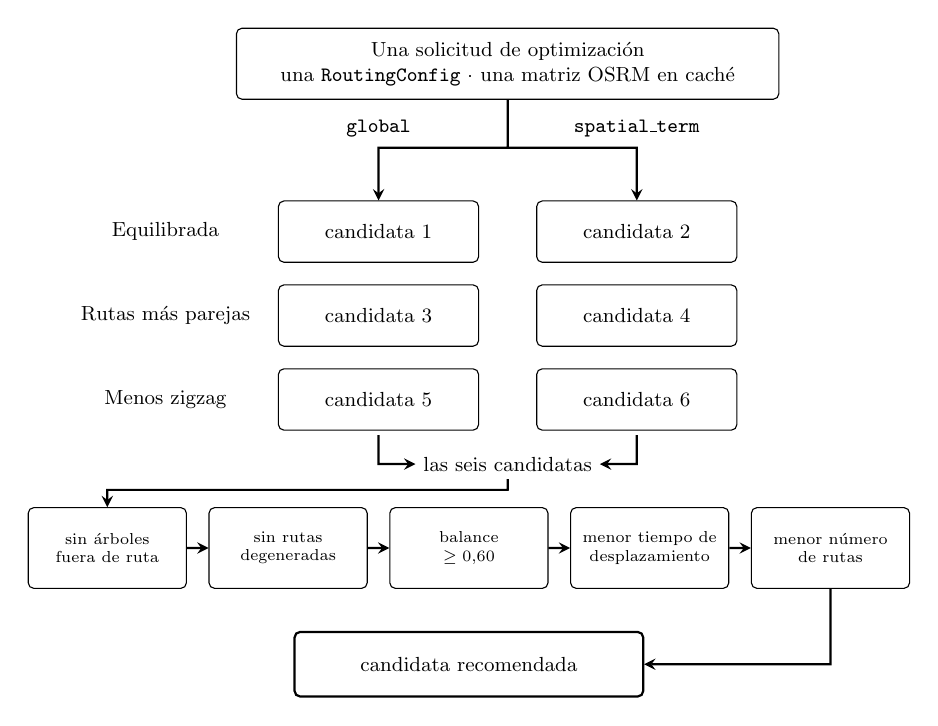
\begin{tikzpicture}[
      scale=0.82, transform shape,
      cab/.style={font=\small},
      celda/.style={draw, rounded corners=2pt, align=center, font=\small,
                    minimum width=3.1cm, minimum height=0.95cm},
      origen/.style={draw, rounded corners=2pt, align=center, font=\small,
                     minimum width=8.4cm, minimum height=1.1cm},
      paso/.style={draw, rounded corners=2pt, align=center, font=\scriptsize,
                   minimum width=2.45cm, minimum height=1.25cm},
      final/.style={draw, thick, rounded corners=2pt, align=center, font=\small,
                    minimum width=5.4cm, minimum height=1.0cm},
      flujo/.style={->, >=stealth, thick}
    ]
    \node[origen] (cfg) at (3.6,2.9)
      {Una solicitud de optimización\\ una \texttt{RoutingConfig} · una matriz OSRM en caché};

    \node[cab] at (1.6,1.9) {\texttt{global}};
    \node[cab] at (5.6,1.9) {\texttt{spatial\_term}};
    \node[cab, align=right] at (-1.7,0.3)  {Equilibrada};
    \node[cab, align=right] at (-1.7,-1.0) {Rutas más parejas};
    \node[cab, align=right] at (-1.7,-2.3) {Menos zigzag};

    \node[celda] (c1) at (1.6,0.3)   {candidata 1};
    \node[celda] (c2) at (5.6,0.3)   {candidata 2};
    \node[celda] (c3) at (1.6,-1.0)  {candidata 3};
    \node[celda] (c4) at (5.6,-1.0)  {candidata 4};
    \node[celda] (c5) at (1.6,-2.3)  {candidata 5};
    \node[celda] (c6) at (5.6,-2.3)  {candidata 6};

    \draw[flujo] (cfg.south) -- (3.6,1.6) -- (1.6,1.6) -- (c1.north);
    \draw[flujo] (3.6,1.6) -- (5.6,1.6) -- (c2.north);

    \node[cab] (todas) at (3.6,-3.3) {las seis candidatas};
    \node[paso] (p1) at (-2.6,-4.6) {sin árboles\\ fuera de ruta};
    \node[paso] (p2) at (0.2,-4.6)  {sin rutas\\ degeneradas};
    \node[paso] (p3) at (3.0,-4.6)  {balance\\ $\geq 0{,}60$};
    \node[paso] (p4) at (5.8,-4.6)  {menor tiempo de\\ desplazamiento};
    \node[paso] (p5) at (8.6,-4.6)  {menor número\\ de rutas};

    \draw[flujo] (1.6,-2.85) -- (1.6,-3.3) -- (todas.west);
    \draw[flujo] (5.6,-2.85) -- (5.6,-3.3) -- (todas.east);
    \draw[flujo] (todas.south) -- (3.6,-3.7) -- (-2.6,-3.7) -- (p1.north);
    \draw[flujo] (p1) -- (p2);
    \draw[flujo] (p2) -- (p3);
    \draw[flujo] (p3) -- (p4);
    \draw[flujo] (p4) -- (p5);

    \node[final] (rec) at (3.0,-6.4) {candidata recomendada};
    \draw[flujo] (p5.south) -- (8.6,-6.4) -- (rec.east);
  \end{tikzpicture}
  \caption{Abanico de producción y criterio lexicográfico de selección.}
  \label{fig:abanico}
\end{figure}

% ---- 3.4 -------------------------------------------------------
\section{IMPORTACIÓN Y SELECCIÓN DE FUENTES LEGADAS}
\label{sec:legacy}

Las dos bases de datos que dejaron las iteraciones anteriores, descritas en la
Sección~\ref{sec:estado-actual}, se incorporan como fuentes de importación, identificadas por el
campo \texttt{source} del modelo \texttt{Tree}.

% Orden cronológico confirmado por los dumps de las bases (migraciones y muestras): legacy_app
% (esquema arbocensus_app_*, muestras por QR) es la más antigua: génesis de base 2021-10 y capturas
% de terreno desde 2021-10; mapea a la app de censado inicial (repo mrecabarren/arbocensus).
% legacy_api (arbocensus_api_app_*, posición/especie explícitas, real_tree_id) es posterior: génesis
%  2023-06 y capturas desde 2023-06; NO corresponde a la ludificación 2023 (fastAPI, modelos
% badge/score/campaign, sin datos de identificación de árboles). La asignación de cada base a una
% MEMORIA concreta sigue siendo inferencia por esquema (no consta en las fuentes), por lo que el
% texto cita ambas memorias en conjunto; pero el orden relativo app-antes-que-api sí está respaldado
% por los timestamps de los dumps. Por eso se presenta primero legacy_app.
\begin{enumerate}
  \item \texttt{legacy\_app} (esquema \texttt{arbocensus\_app\_*}): la más antigua, base de la
        aplicación de censado previa ---una aplicación web orientada a dispositivos móviles---,
        donde el árbol no tiene una posición canónica sino un conjunto de muestras
        (\textit{samples}) tomadas en terreno, cada una con su propia lectura de GPS. La posición de
        cada árbol se reconstruye como la mediana de las latitudes y longitudes de sus muestras,
        agrupadas por
        código QR, descartando las lecturas sin coordenada, las que caen fuera del rango de Chile
        continental ---con lo que se eliminan las lecturas de GPS fallidas, que la aplicación previa
        registraba como coordenada nula--- y los códigos QR compuestos solo de ceros. Se emplea la
        mediana y no el promedio por su robustez frente a lecturas de GPS atípicas. De este modo se
        obtienen $12\,941$ árboles con posición utilizable, sobre un total de $17\,208$ muestras.
  \item \texttt{legacy\_api} (esquema \texttt{arbocensus\_api\_app\_*}): posterior a la anterior, 
        aporta $429$ árboles con posición explícita y especie, organizados en áreas pertenecientes a
        campañas de censo.
\end{enumerate}

Ambas fuentes se solapan geográficamente, por lo que se descarta el árbol de \texttt{legacy\_app}
que se encuentre a $5$\,m o menos de uno de \texttt{legacy\_api} ---se conserva este último, que
aporta especie y área---. La proximidad es el único criterio de correspondencia disponible, dado
que las fuentes no comparten un identificador común. El umbral de $5$\,m es deliberadamente
conservador: la literatura reporta para receptores de teléfono en entorno urbano errores
horizontales medios de $7$--$13$\,m \citep{merry2019smartphone}, mayores que el propio umbral, de
modo que el criterio deja pasar duplicados antes que fusionar dos ejemplares distintos que caen
cerca; se prefiere ese error porque un árbol duplicado cuesta una visita redundante, mientras que
uno fusionado por error desaparece del catastro. El explorador expone así $13\,319$ árboles
importables: $429$ de \texttt{legacy\_api} y $12\,890$ de \texttt{legacy\_app}. Ese es el universo
disponible; el \textit{dataset} de $n = 1\,607$ árboles con que se evalúa el sistema
(Capítulo~\ref{cap:resultados}) es una instancia congelada de ese universo, elegida por
reproducibilidad, y no su totalidad. El acceso a las bases legadas es estrictamente de solo lectura
(RE-03).

\subsection{Selección previa a la creación del \textit{dataset}}

La decisión de diseño central de este módulo es que la importación no crea un \textit{dataset} de
forma inmediata. La primera versión del importador de esta iteración traía áreas completas a ciegas
(mediante CSV/JSON), lo que resulta inadecuado: el usuario no sabe, antes de importar, qué árboles
trae un área, cuáles ya están en el sistema ni si el conjunto resultante corresponde al territorio
que efectivamente quiere censar. El flujo se divide por ello en dos etapas: primero explorar y
seleccionar, y solo después materializar el \textit{dataset} con la selección confirmada.

La exploración se sirve de dos \textit{endpoints} de solo lectura: uno lista las áreas de censo con
su campaña, su número de árboles y su polígono ---la fuente almacena las áreas como listas de
vértices, por lo que el polígono se reconstruye y la pertenencia de cada árbol a un área se
determina por inclusión punto-en-polígono, no por una clave foránea que la fuente no provee---, y
el otro devuelve el arbolado de ambas fuentes con su posición, su especie, el área que lo contiene
y una marca \texttt{already\_imported}. El explorador admite filtrar por estado y por fuente de
origen, y permite reincorporar un árbol ya importado en otro \textit{dataset} (RF-25).

La materialización ocurre en un único paso transaccional que recibe el nombre del \textit{dataset}
y la lista de árboles seleccionados, identificados por el par (\texttt{source},
\texttt{external\_id}) y no por un identificador plano: al coexistir dos fuentes con espacios de
identificadores independientes, un \texttt{external\_id} por sí solo es ambiguo. El
\textit{endpoint} crea el \texttt{Dataset}, sus \texttt{Tree} y el histórico de observaciones
asociado (Sección~\ref{sec:recenso}) dentro de una misma transacción, de modo que un fallo parcial
no deja \textit{datasets} a medio poblar. Un \textit{endpoint} auxiliar importa un área completa o
la fuente entera sin selección previa; no forma parte del flujo del usuario y se conserva como
atajo programático para construir \textit{datasets} reproducibles en los experimentos del
Capítulo~\ref{cap:resultados}.

\subsection{Mapa de selección}

La interfaz de selección presenta sobre un mapa \textit{Leaflet} la totalidad del arbolado legado y
los polígonos de las áreas de censo ---la unidad con que se organizó la operación histórica, que el
administrador reconoce y que el Capítulo~\ref{cap:resultados} identifica como la escala natural del
motor---. Cada árbol se dibuja como un marcador cuyo color codifica su estado: disponible,
seleccionado o ya importado; estos últimos no son interactivos, lo que hace imposible seleccionar
dos veces el mismo árbol. La selección puede componerse mediante tres mecanismos combinables:

\begin{enumerate}
  \item Por área: al hacer clic sobre el polígono de un área se alternan de una vez todos los
        árboles contenidos en ella.
  \item Por región trazada: el administrador traza sobre el mapa ---como polígono de vértices
        editables o como rectángulo--- la región que quiere censar, y se agregan a la selección
        todos los árboles contenidos en ella, con independencia del área a la que pertenezcan.
        Pueden coexistir varias regiones, cuya unión constituye la selección.
  \item Por árbol individual: el clic sobre un marcador agrega o quita ese árbol de la selección.
\end{enumerate}

Un panel lateral mantiene visible la selección acumulada y permite la deselección manual de
cualquier árbol, de forma que los tres mecanismos anteriores actúan como brochas gruesas que el
usuario refina antes de confirmar. Solo al confirmar ---indicando el nombre del \textit{dataset}---
se emite la solicitud de creación. El resultado es que el recorte territorial del censo es una
decisión explícita del administrador, tomada sobre la evidencia cartográfica, y no una consecuencia
de cómo estaban organizadas las áreas en el sistema anterior.\footnote{Ver
\hyperref[anx:capturas]{Anexo 6}.}

% ---- 3.5 -------------------------------------------------------
\section{RE-CENSO Y REGISTRO DE OBSERVACIONES}
\label{sec:recenso}

Un censo de arbolado urbano no es un evento único sino un proceso recurrente: el valor del catastro
está en la comparación del estado de un árbol entre campañas sucesivas. El modelo de datos separa
por ello dos conceptos que suelen confundirse. El \texttt{RouteStop} es una unidad de trabajo:
pertenece a una ruta, tiene una secuencia y un estado de avance (\texttt{pending}, \texttt{visited},
\texttt{skipped}), y su vida termina cuando la ruta se completa. La \texttt{TreeObservation}, en
cambio, es un hecho histórico: registra el estado en que se encontró un árbol en un instante dado y
no caduca. Un árbol acumula tantas observaciones como veces haya sido censado, y su relación con el
\texttt{RouteStop} que la originó es opcional (\texttt{SET\_NULL}), precisamente porque una
observación debe sobrevivir a la eliminación del plan de rutas que la produjo, e incluso puede no
provenir de ruta alguna, como es el caso de las observaciones importadas de las fuentes legadas.

Cada \texttt{TreeObservation} registra el estado del árbol (\texttt{alive}, \texttt{removed},
\texttt{not\_found}, \texttt{other} o \texttt{unknown}), una fotografía, notas libres, el autor y la
marca temporal de la observación. El estado \texttt{unknown} es deliberado: permite ingresar una
observación cuyo estado no consta ---típicamente, un registro histórico importado--- sin forzar una
afirmación que la fuente no respalda.

\subsection{Captura en terreno}

En el portal del censista (Sección~\ref{sec:ui}), toda parada genera una observación, tanto si el
árbol se visita como si se omite. Al registrar una visita, el censista selecciona el estado del
árbol y captura una fotografía. La fotografía es obligatoria cuando el estado declarado afirma haber
visto el árbol ---\texttt{alive} o \texttt{removed}---: la interfaz mantiene la confirmación
deshabilitada mientras no se haya tomado, y el servidor rechaza con un código 400 la petición que
llegue sin ella. La validación se duplica de forma deliberada en ambos extremos, porque un control
que solo existe en el cliente es evadible con cualquier herramienta HTTP y no constituye una
garantía del sistema. 

La excepción es el estado \texttt{not\_found}, que se registra como visita pero sin exigir imagen,
por la razón evidente de que no hay árbol que fotografiar; lo mismo vale para las omisiones, que se
tratan más abajo. La regla es entonces que se exige evidencia gráfica de toda afirmación positiva
sobre el estado de un árbol, y no de la constatación de su ausencia.

Conviene precisar el alcance de esa garantía. La fotografía es la evidencia documental de la
observación, pero no acredita por sí sola que el censista haya estado frente al árbol correcto: no
se verifica su contenido, ni sus metadatos de posición, ni el instante de captura. El control de
proximidad de $30$\,m que la interfaz aplica antes de habilitar el registro (Sección~\ref{sec:ui})
tampoco cierra esa brecha: se evalúa en el cliente, ofrece forzar el registro cuando la señal de
GPS es imprecisa y el servidor acepta las coordenadas que reciba. Es deliberadamente una guía y no
una compuerta, porque bloquear el registro ante una señal de GPS fallida costaría la observación
completa de la jornada. La trazabilidad que el sistema sí garantiza es de autoría y momento: cada
observación queda ligada al usuario que la registró y a su marca temporal, y no puede alterarse
retroactivamente.

La captura se realiza con la cámara del dispositivo desde el propio navegador y la observación
viaja al servidor como \textit{multipart} cuando incluye imagen. Al omitir una parada, el censista
debe indicar un motivo (árbol inexistente, acceso bloqueado u otro) y la fotografía no se exige; el
estado de la observación se deriva del motivo ---\texttt{not\_found} para árbol inexistente,
\texttt{unknown} para el resto---, de modo que incluso una parada omitida deja constancia histórica
de por qué no se pudo censar.

Que la fotografía sea obligatoria es, con todo, una regla de esta iteración y no un requisito que
se derive del propósito del proyecto: el protocolo de censo que fijaría esa exigencia no está
definido ---la misma indefinición que obliga a tratar el tiempo de servicio $s$ como parámetro
(Sección~\ref{sec:flota})---, y la imagen se persiste en el sistema de archivos del contenedor, sin
almacenamiento de objetos ni copia fuera del servidor. Ambas cosas se asumen como limitación y el
Capítulo~\ref{cap:resultados} las retoma como tal.

\subsection{Instantánea del histórico legado}

La importación de una fuente legada no trae solo la posición de los árboles: trae también, en la
misma transacción, sus observaciones previas, que se materializan como \texttt{TreeObservation} con
el campo \texttt{source}, que registra su procedencia. El resultado es que un árbol recién importado
ya llega al sistema con su historial de campañas anteriores, y la primera visita del censista se
registra como una observación más en esa serie ---esto es, como un re-censo y no como un censo
inicial.

El vínculo entre una observación legada y su árbol difiere según la fuente: en \texttt{legacy\_api}
las muestras referencian al árbol directamente, mientras que en \texttt{legacy\_app} lo hacen a
través del código QR físico adherido al árbol. De las fotografías históricas se conserva su URL y
no el archivo, dado que las imágenes residen en el almacenamiento del sistema anterior; las de
\texttt{legacy\_api} son hoy inaccesibles porque el plan de facturación del proyecto que las aloja
está cerrado (Sección~\ref{sec:limitaciones}). El estado se deriva del único campo disponible en el
origen ---si la muestra fue o no completada---, mapeando la muestra completada a \texttt{alive} y
el resto a \texttt{unknown}, en lugar de inferir un estado que la fuente no consigna. La identidad
persistente del árbol entre campañas es el par (\texttt{source}, \texttt{external\_id}), que
\texttt{Tree} conserva en toda importación, de modo que el historial entre campañas se resuelve por
la clave natural y no por el identificador de fila.

% ---- 3.6 -------------------------------------------------------
\section{API REST}
\label{sec:api}

La API REST se implementa con Django REST Framework, con autenticación por \textit{tokens}
\textit{JSON Web Token} (JWT) mediante \textit{djangorestframework-simplejwt}.
Los dos usuarios objetivo de la Sección~\ref{sec:usuarios} se materializan en la API como dos roles:
Administrador (acceso completo) y Censista (lectura de las rutas propias del plan vigente y registro
de visitas). La autorización se resuelve por rol mediante los
permisos propios \texttt{IsAdminRole} e \texttt{IsSurveyorRole}, definidos sobre el campo
\texttt{role} del usuario y no sobre los permisos estándar del \textit{framework}, que validan el
atributo \texttt{is\_staff} de Django ---un concepto ajeno al rol de negocio. La
Tabla~\ref{tab:endpoints} resume los \textit{endpoints} más relevantes.\footnote{Ver \hyperref[anx:api]{Anexo 1}.}

\begin{table}[H]
  \centering
\caption{Grupos de recursos de la API REST.}
  \label{tab:endpoints}
  \small
  \begin{tabularx}{\textwidth}{@{}l l X@{}}
    \toprule
    Grupo &
      Prefijo &
      Propósito \\
    \midrule
    Autenticación &
      \texttt{/api/auth/} &
      \textit{Tokens} JWT, consulta del usuario en sesión y gestión de cuentas de censistas. \\
    \textit{Datasets} &
      \texttt{/api/datasets/} &
      Importación CSV/JSON y desde fuentes legadas, exploración, exportación \textit{GeoJSON} e
      historial de observaciones. \\
    Optimización &
      \texttt{/api/optimization/} &
      Estimación de flota y comprobación de factibilidad, creación de trabajos, \textit{polling} de
      estado, métricas de soluciones y publicación del plan vigente. \\
    Rutas &
      \texttt{/api/routes/} &
      Listado con métricas, exportación \textit{GeoJSON}, asignación de censistas, carga acumulada
      por censista con sugerencia de asignación, ruta propia del censista y registro de visitas y
      omisiones. \\
    \bottomrule
  \end{tabularx}
\end{table}

Los grupos \textit{Datasets} y Optimización son exclusivos del rol Administrador, al igual que la
administración de cuentas dentro del grupo Autenticación; el resto de ese grupo ---obtención y
renovación del \textit{token} y consulta de la sesión propia--- lo utilizan ambos roles. Rutas es el
único grupo cuyas operaciones de negocio comparten los dos, con el censista restringido a su propia
ruta vigente.

% ---- 3.7 -------------------------------------------------------
\section{INTERFAZ DE USUARIO Y FLUJOS DE OPERACIÓN}
\label{sec:ui}

La interfaz se implementa como una \textit{Single Page Application} con \textit{React}~18 y Vite;
el estado de servidor se gestiona con \textit{React Query}, el de sesión con Zustand y los mapas
emplean \textit{Leaflet} sobre teselas de \textit{OpenStreetMap} \citep{openstreetmap}. La
aplicación distingue dos experiencias según el rol: el panel de administración y el portal del
censista.

El panel de administración comprende cinco etapas:

\begin{enumerate}
  \item Sesión. El administrador inicia sesión y obtiene un \textit{token} JWT.
  \item Constitución del \textit{dataset}. Importa un archivo CSV o selecciona el arbolado sobre el
        mapa de fuentes legadas (Sección~\ref{sec:legacy}); en ambos casos el resultado se visualiza
        como puntos sobre el mapa.\footnote{Ver \hyperref[anx:capturas]{Anexo 6}.}
  \item Configuración y lanzamiento. Configura $T_{\min}$, $T_{\max}$ y el tiempo de servicio, y
        lanza el trabajo. El formulario no expone ni la estrategia ni los coeficientes del objetivo:
        una sola solicitud despliega el abanico de seis combinaciones de la
        Sección~\ref{sec:abanico}. La estimación de flota y la comprobación de factibilidad se
        consultan a medida que el administrador escribe: las advertencias se muestran junto al
        formulario y los bloqueos inhabilitan el botón de lanzamiento.
  \item Monitoreo. \textit{React Query} consulta el estado del trabajo cada 3 segundos y detiene
        las consultas al alcanzar un estado terminal o superar 15 minutos.
  \item Presentación, recomendación y publicación. Las rutas resultantes se presentan como
        polilíneas coloreadas sobre la red peatonal real, y las seis soluciones se listan como
        candidatas a plan ordenadas por el criterio lexicográfico de la
        Ilustración~\ref{fig:abanico}. Sobre ese orden se aplica una regla de estabilidad: si el
        par de control ---perfil \texttt{default} con estrategia \texttt{spatial\_term}--- supera
        las mismas compuertas que el primero y su desplazamiento no se aparta de él más de un
        $3$\,\%, se recomienda el control, con el fin de que un empate dentro del ruido del
        \textit{solver} no cambie la recomendación entre corridas; una candidata cuyo
        desplazamiento difiere de la recomendada en menos de ese mismo margen se rotula como empate
        técnico. La recomendación no es vinculante: el administrador publica la candidata que
        estime conveniente. Publicado el plan, \texttt{suggest\_assignment} propone una asignación
        de rutas a censistas que reduce el déficit de carga acumulado entre campañas, y el
        administrador la acepta o la modifica ruta por ruta.
\end{enumerate}

El panel de optimización del \textit{dataset} (\texttt{/admin/datasets/\{id\}}) muestra en el mapa
la solución recomendada sobre la red peatonal; el panel lateral concentra la configuración de
parámetros ($T_{\min}$, $T_{\max}$ y tiempo de servicio), el estado de la última optimización y la
lista de candidatas a plan ordenadas por el criterio de selección, cada una con la caminata
adicional que cuesta respecto de la recomendada. El clic sobre un marcador del mapa despliega el
historial de observaciones de ese árbol, lo que permite al administrador verificar si ya fue censado
antes de lanzar la optimización. Cada candidata de la lista resume tres métricas ---número de
rutas, tiempo de caminata y puntaje de balance--- y destaca en cuáles de ellas es la mejor de la
corrida; los árboles que quedan fuera de ruta, las rutas degeneradas y el balance bajo el umbral no
se presentan como cifras sino como advertencias en lenguaje llano, porque son condiciones que
descalifican a la candidata y no magnitudes que el administrador deba ponderar. Como dos corridas
con parámetros temporales distintos no son comparables entre sí, la lista muestra una sola corrida
a la vez y un selector permite alternar entre ellas.

Publicado el plan, el administrador supervisa el avance del censo desde la pestaña de progreso: el
tablero resume el porcentaje de árboles censados, omitidos y pendientes, los sitúa sobre el mapa
según su estado y desglosa el avance por ruta y por censista, de modo que se identifican qué rutas
van retrasadas. Esta vista realiza RF-19 y RF-20.

El portal del censista (\texttt{SurveyorRoutePage}) es una vista \textit{mobile-first} orientada al
trabajo en terreno. Recupera únicamente las rutas del plan vigente asignadas al usuario y presenta
las paradas en orden secuencial estricto: una parada solo puede marcarse como visitada cuando las
anteriores ya lo han sido. La ubicación del censista se sigue mediante la API de geolocalización del
navegador y se calcula la distancia de \textit{haversine} \citep{sinnott1984virtues} a la parada
activa; el registro de visita se habilita al entrar en un radio de proximidad de 30\,m, con la
opción de forzar el registro (\textit{«Registrar de todos modos»}) cuando la señal GPS es imprecisa.
Tanto la visita como la omisión de una parada generan una observación del árbol, con captura
fotográfica y estado, según el diseño descrito en la Sección~\ref{sec:recenso}. Cada parada ofrece
un enlace directo (\textit{deep-link}) a la navegación peatonal de Google Maps. La pantalla se
mantiene encendida durante el recorrido mediante la \textit{Screen Wake Lock API}, y una cola de
operaciones \textit{offline} básica ---persistencia del cliente de \textit{React Query} en
\textit{IndexedDB}, único almacén del navegador capaz de conservar el objeto \texttt{File} de la
fotografía pendiente--- permite que el registro realizado sin conexión se sincronice al recuperar
la red.

Su vista general presenta el mapa de la ruta con las paradas numeradas según
\texttt{RouteStop.sequence}, la parada activa con su distancia y el estado del registro, y la lista
de paradas, con las posteriores a la activa bloqueadas hasta completar la anterior.

% ---- 3.8 -------------------------------------------------------
\section{VERIFICACIÓN Y VALIDACIÓN}
\label{sec:verificacion}

El comportamiento descrito en este capítulo ---y con él los requisitos funcionales comprometidos en
la Sección~\ref{sec:requisitos-funcionales}--- se sostiene sobre una suite de pruebas automatizadas
que se ejecuta en cada integración de cambios: 524 funciones de prueba de \textit{backend} en 47
archivos y 304 casos de \textit{frontend} en 44, acompañados de análisis estático
---\textit{Ruff}, \textit{Pyright} y \textit{ESLint}--- y de los flujos de integración y entrega
continuas que encadenan análisis, pruebas y construcción, y que actualizan el servidor ante cada
\textit{push} a la rama \texttt{production}
(Sección~\ref{sec:despliegue-produccion}).\footnote{Ver \hyperref[anx:trazabilidad]{Anexo 5}.}

Las pruebas del \textit{backend} se apoyan en \textit{pytest} con una base de datos PostGIS real y
no en dobles de prueba, de modo que las consultas geográficas y las restricciones de unicidad
parcial descritas en la Sección~\ref{sec:modelo-datos} se ejercitan tal como operan en producción.
Las del motor de optimización comprueban propiedades del modelo y no valores concretos ---que
dependerían del corte por reloj de pared del \textit{solver}---:

\begin{enumerate}
  \item el depósito ficticio no aparece en ninguna ruta extraída;
  \item la suma de paradas más descartes cubre el conjunto de árboles;
  \item la clave de caché de la matriz es independiente del orden de consulta;
  \item ninguna ruta excede $T_{\max}$ en la aritmética entera del \textit{solver}.
\end{enumerate}

Corresponde acotar el alcance de esta verificación. No existen pruebas automatizadas de extremo a
extremo: los flujos completos de administrador y de censista se comprueban por partes, nunca
encadenados sobre el sistema en pie, y esta memoria no reporta una cifra de cobertura de código.
Sobre todo, lo que se verifica es que el sistema hace lo que su diseño dice: la validación con
usuarios reales ---una jornada de censo con censistas en terreno--- queda fuera del alcance de esta
iteración y es la comprobación que ninguna suite de pruebas sustituye.

A esta verificación se suma un compromiso distinto: la reproducibilidad de las cifras del
Capítulo~\ref{cap:resultados}. Como la búsqueda se corta por reloj de pared y la biblioteca no
permite fijar una semilla (RE-04, RE-05), el compromiso es que un tercero pueda regenerar las
cifras publicadas desde el mismo comando de gestión y la misma instancia congelada y versionada, no
que el \textit{solver} sea determinista. Reproducir una cifra tampoco significa que la solución sea
óptima: acredita el procedimiento, no la calidad del plan.
